\section{Tuesday, April 2nd}
\subsection{Logistics}
\begin{itemize}
    \item Review Reviews due Today
    \item Project Draft due next week, Thursday
    \item Reading (Ch. 4), post by Thurs
    \item Quiz 6 on Thurs: First half of chapter  4.1, 4.2 (Entropy rates and markov chains). Note that 4.4 and Mixing Inequalities (and thermodynamics) will be on the next quiz (not this upcoming one).
\end{itemize}

\subsection{Why cover Stochastic Processes}
If our end goal is to talk about communication and channels, why divert to processes?

\begin{shaded}
Answer: Stochastic Processes are a natural model for the process that generates the messages we want to send. Many messages like audio, video, text (sequence of characters with a distribution of next possible characters as opposed to future character popping out of nowhere), etc can be modeled as a process evolving over time.
\end{shaded}

This helps induce specific structural assumptions on joint dist. of possible messages, where assumptions $\Rightarrow$ results.

\subsection{Entropy Rates Review}
Stochastic Processes, $\cX$ ensemble (both the space of what you can send and their respective probabilities), $\{X(t)\}_t\sim$ joint distribution.


$$
H[\cX] = \lim_{n \rightarrow \infty} \frac{1}{n} H[X^{(n)}]
$$ where $X^{(n)} = \{X_1, X_2, \ldots, X_n \}, X_j = X(t_j)$

if there is, each time I take a step Iadd additional randomness. Thus:
\begin{shaded}
Entropy increases as $n\to\infty$.
\end{shaded}

This is the sample-wise uncertainty/randomness in the trajectory (for long trajectories). This has a dual perspective if you approach the problem geometrically. As we have longer processes, the stochastic process should grow as a fn of $n$ as $n$ increases.

\begin{figure}[H]
    \centering
    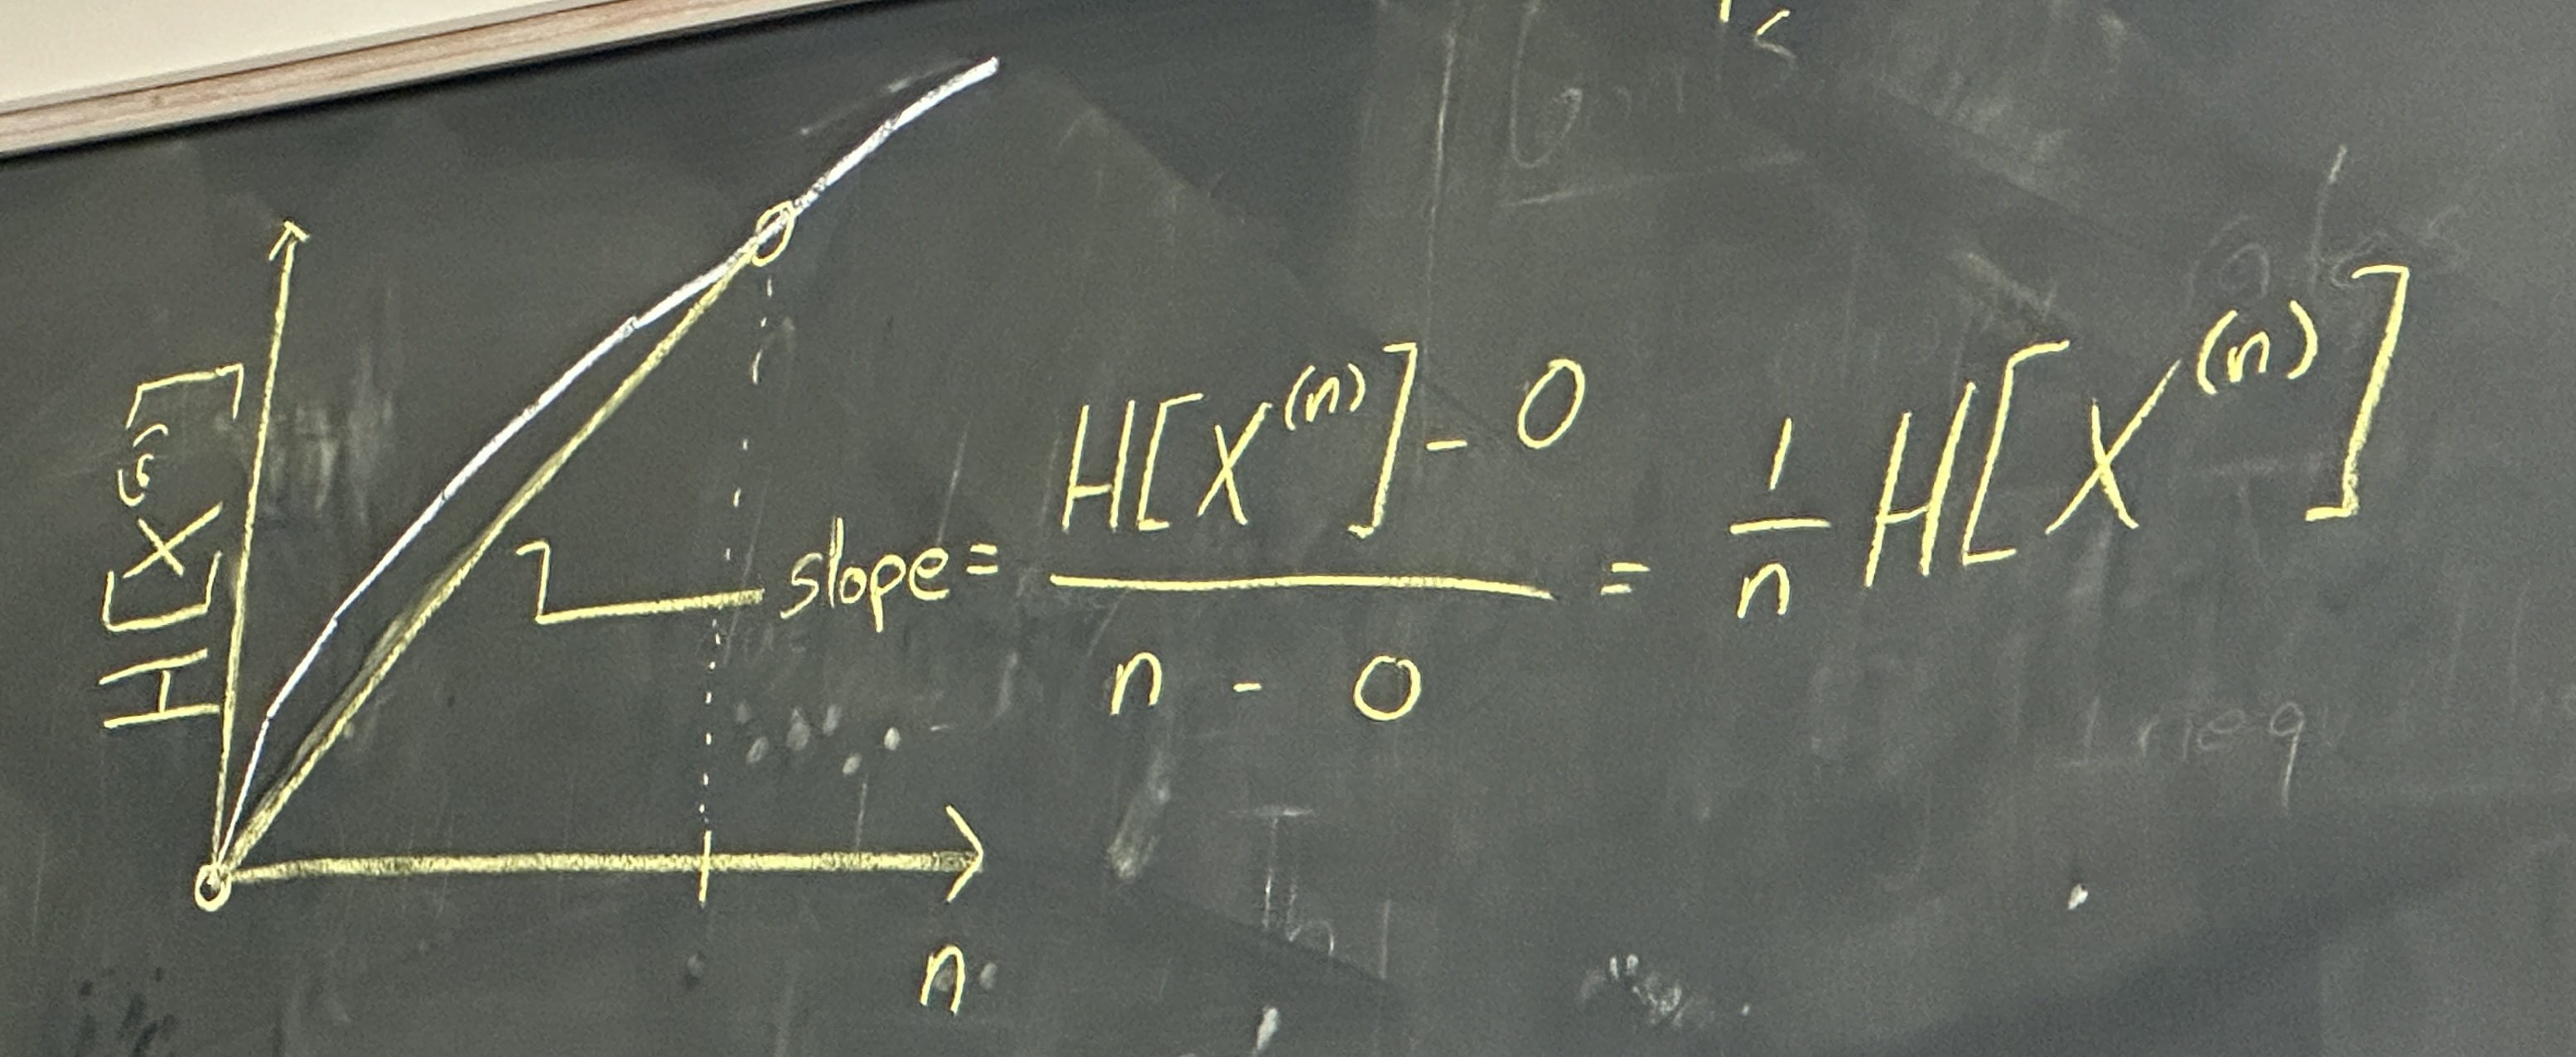
\includegraphics[scale=0.15]{lectures/wk11/img/entropy_increasing.jpg}
    \caption{We examine the secant line}
    \label{fig:enter-label}
\end{figure}

We use the word rate since this is the long term rate of growth in the joint entropy of a long trajectory, $H[X^{(n)}]$.

\begin{itemize}
\item $H[X_{n+1} \mid X^{(n)}]$
\item 
    \begin{align*}
    H[X^{(n+1})] - H[X^{(n)}] 
        &= (H[X^{(n)}]+H[X_{n+1}\mid X^{(n)}]) - H[X^{(n)}]
    \\
        &= H[X_{n+1}\mid X^{(n)}]
    \end{align*}
\end{itemize}

\subsubsection{Alternate defn. of Entropy Rate}
\begin{align*}
    H'[\cX]
    &= \lim_{n\to\infty} H[X_{n+1} \mid X^{(n)}]
\end{align*}

If $\cX$ is stationary $\implies H[\cX]=H'[\cX]$. A stationary process means if I sample at a sequence of time, the joint distributions would not change under time (time-invariance).

\subsection{Application of Entropy Rate}
Recall how we studied compression earlier in the semester.

We have messages $\{X(t_j)\}_{j=1}^n, X^{(n)}\sim \cX$.

We have Code: $C(X^{(n)})\to$ string of $d$-ary characters.
\begin{itemize}
    \item ($C_j\in \{\text{instantaneous codes $\cX$}\}$)
\end{itemize}
Note that `dits' is the equivalent of `bits' for $d$-ary character as opposed to binary.

$L(C)=\E_{X^{(n)}}[|c(x^{(n)})|], \quad L^*(\cX)=\min_{c\in C}\{L(x)\}\in [H_d[X^{(n)}], H_d[X^(n)] + 1]$.

$L^*$ should be growing as we try to encode longer messages, as we increase $n$.

This leads to $L_n^*(\cX) = \frac1n L(\cX)$.

$$\lim_{n\to\infty} \frac1n L^*(\cX)\in\lim_{n\to\infty} \frac1n(H_d[X^{(n)}] + [0, 1]) \to H_d[\cX] + \cO\left(\frac1n\right)$$

\subsection{Innovation Rates}
\begin{align*}
\text{Entropy Rate of process } 
&= H[\cX] 
\\
&= \text{ a minimum (best rate), the number of dits per sample needed 
}
\\
&
\quad\quad
\text{
on average to specify a trajectory.}\\
&= \text{ new info needed to specify $X_{n+1}\mid X^{(n)}$} (on average)
\end{align*}

Everything above is in-scope for Quiz 6.

\hrulefill

Everything below is in-scope for Quiz 7:
\subsection{Mixing Inequalities (Markov Chains)}
\begin{itemize}
    \item $\cX$ is a (Discrete-Time) M.C., $X(0)\sim p_0, Y(0)\sim q_0, X_n\sim p_n, Y_n\sim q_n$
\end{itemize}
\begin{enumerate}
    \item $D(p_{n+1} \| q_{n+1}) \leq D(p_n \| q_n)$, so $\{D(p_n\|q_n)\}$ is monotonically nonincreasing. `If they follow the same rules, they should forget how they were initialized.'
    
    Moral: 
    \begin{shaded}
    The process \textit{mixes}: the cdtl. distribution of the current state gets more similar to the cdtl. distro. initialized differently.
    \end{shaded}
\end{enumerate}
\begin{proof}
Like most proofs in this class, if it does not involve Jensen's/convexity, we use Chain Rule:
\begin{align*}
D(p_{X_{n+1}, X_n} \| q_{Y_{n+1}, Y_n}) 
&= \begin{cases}
    \text{Past:}
    & 
    D(\underbrace{p_{X_n}}_{p_n} \| \underbrace{q_{Y_n}}_{q_n}) + \underbrace{D(p_{X_{n+1} \mid X_n} \| q_{Y_{n+1}\mid Y_n})}_{0 \text{ since they follow the same transition probabilities}}
    \\
    \text{Future:}
    & 
    D(%\underbrace
    {p_{{n+1}}}
    %_{p_n}
    \| %\underbrace
    {q_{{n+1}}}
    %_{q_n}
    ) + \underbrace{D(p_{X_{n} \mid X_{n+1}} \| q_{Y_{n}\mid Y_{n+1}})}_{\geq0}
\end{cases}
\\
&= \begin{cases}
    \text{Past:}
    & 
    D(p_n\|q_n)
    \\
    \text{Future:}
    & 
    D(%\underbrace
    {p_{{n}}}
    %_{p_n}
    \| %\underbrace
    {q_{{n}}}
    %_{q_n}
    ) 
    - \underbrace{\ldots}_{\geq0}
    + \underbrace{D(p_{X_{n} \mid X_{n+1}} \| q_{Y_{n}\mid Y_{n+1}})}_{\geq0}
\end{cases}
\\
D(%\underbrace
    {p_{{n+1}}}
    %_{p_n}
    \| %\underbrace
    {q_{{n+1}}}
    %_{q_n}
    )
    &\leq 
    D(%\underbrace
    {p_{{n}}}
    %_{p_n}
    \| %\underbrace
    {q_{{n}}}
    %_{q_n}
    ) 
\end{align*}
\end{proof}

\subsection{What does it mean if your MC is Stationary}
It means you are irreducible and aperiodic and finite. Then $\exists p_s$ which is a stationary distributions. If you initialize $Y$ from the stationary then you stay there. Thus $D(p_{n+1}\| p_{s})\leq D(p_{n}\| p_{s})$, and $p_n\stackrel{n\to\infty}\to p_s\quad\forall p_s$.

\begin{equation}
    D(p_n\| p_{s}) \stackrel{n\to\infty}\to 0, \quad
    D(p_n\| q_{n}) \stackrel{n\to\infty}\to 0
\end{equation}

\subsection{Linkages to Data Processing}
\begin{enumerate}
    \item[2.] $I[X_{1} \| X_{n+1}) = I[X_{n+1} \| X_{1}] \leq I[X_1; X_n]=I[X_n; X_1]$, so: $\{I[X_1\|X_n]\}$ is monotonically non-increasing.

The longer you let this process run, the less information you have about the past.

The longer you let a MC run, the less information you have about where it started: ``the process forgets where it started''.
    \begin{itemize}
        \item Then: $H[X_1\mid X_{n+1}] \geq H[X_1\mid X_{n}]$.
        \item And if stationary: $H[X_{n+1} \mid X_1] \geq H[X_n \mid X_1]$. You will ultimately forget \textbf{everything} about where you started. It carries \textit{no} information about the far past.
    \end{itemize}
\end{enumerate}

\subsection{The second law of Thermodynamics}
\begin{itemize}
    \item $H[X_1\mid X_{n+1}] \geq H[X_1\mid X_n]?$

    Recall $I[A; B] = H[A] - H[A\mid B] = H[B] - H[B\mid A]$.
    
    DPI (Data Processing Inequality): $I[X_1; X_{n+1} \leq I[X_1; X_n].$
    
    $H[X_1] - H[X_1 \mid X_{n+1}]\leq
    H[X_1]  - H[X_1 \mid X_{n}]
    \implies
    $ 
    $ - H[X_1 \mid X_{n+1}]\leq
      - H[X_1 \mid X_{n}]
    $ 
    $  
    \implies
    H[X_1 \mid X_{n+1}]\geq
       H[X_1 \mid X_{n}]
       .
       \hfill\square
    $ 

    \item $H[X_{n+1}\mid X_1] \geq H[X_n\mid X_1]?$

    DPI: $I[X_{n+1}; X_{1} \leq I[X_n; X_1]$.
    
    $H[X_{n+1}] - H[X_{n+1} \mid X_{1}]
    \leq
    H[X_{n}] - H[X_{n} \mid X_{1}]
       .
    $ 

    If stationary by DPI: 
    \begin{align*}
        H[X_{n+1}] - H[X_{n+1} \mid X_1] &\leq H[X_n] - H[X_n \mid X_1] \\
        H[p_{x_{n+1}}] - H[X_{n+1}] &\leq H[p_{x_{n+1}}] - H[X_n \mid X_1] \\
        H(p_s) - H[X_{n+1} \mid X_1] &\leq H(p_s) - H[X_n \mid X_1] \\ 
        H[X_{n+1} \mid X_1] &\geq H[X_n \mid X_1]
    \end{align*}

    $H[X_{n+1}\mid X_1]
    \geq
    H[X_{n}\mid X_1]
    \hfill\square$
    
\end{itemize}



